\documentclass{article}
\usepackage{amsmath, graphicx}
\usepackage[margin=1.2in]{geometry}
\author{Wenqi He}
\title{CS 4235 Project 1}
\begin{document}
\maketitle
\section{}
\subsection*{a}
The stack starts from the highest addresses (right before the command-line arguments and environment variables) in the address space and grows towards lower memory addresses. Whenever a function is called, a new stack frame, which contains the arguments passed into the function, current \texttt{\$eip} ( the return address, which points at the next instruction to be executed after the callee returns), current \texttt{\$ebp} pointing at the calling frame,  local variables, etc. (see diagram 1.a), is pushed onto the stack. Local variables are placed right before the location addressed by \texttt{\$ebp}. Arguments are placed right after the return address. When a function returns, the return address stored on the current stack frame will be used to jump back to the calling function. If the length of a variable can cause misalignment, it would be padded so that it takes up exactly a multiple of the word size.
\subsection*{b}
\begin{verbatim}
#include<stdio.h>

int main(char* args} {
    echo();
}

void echo() {
    char buffer[4];
    gets(buffer);
    printf("%s\n", buffer);
}
\end{verbatim}
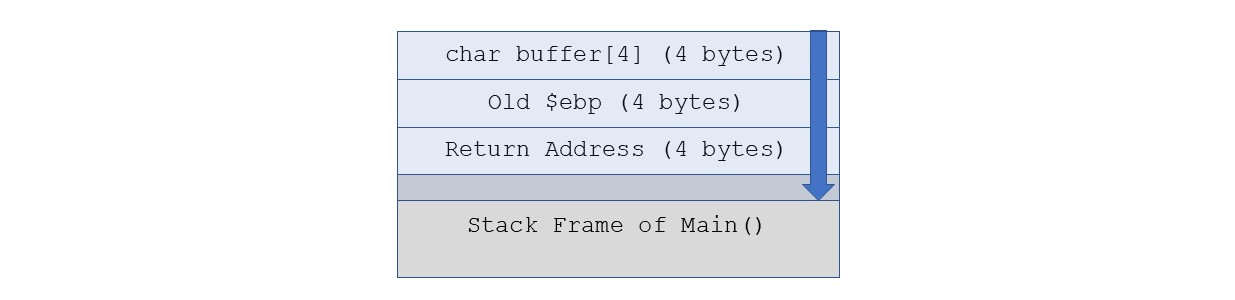
\includegraphics[width=\textwidth]{1b.jpg}\\
Function \texttt{echo()} read a string from standard input and puts it in a buffer of size 4 bytes on the stack. Typing in a string with more than 4 characters will cause buffer overflow. It takes string of 12 characters to reach and overwrite the return address.

\section{}
\subsection*{a}
The heap is located at the lowest memory addresses, right after the text segemnt, initialized data segment and uninitialized data segment. It grows towards higher memory addesses. It starts from the opposite side of the address space and grows in the opposite direction compared to the stack.
\subsection*{b}
b.
\begin{verbatim}
#include<stdio.h>
#include<string.h>

typedef struct person {
    void (*greet)(char *name);
    char name[4];
} person;

void greeting_func(char *name) {
    printf("Hi, my name is %s\n", name);
}

int main(char* args} {
    person_a = malloc(sizeof(person));
    person_b = malloc(sizeof(person));
    person_a->greet = greeting_func;
    person_b->greet = greeting_func;
    gets(person_a->name);
    gets(person_b->name);
    person_a->greet(person_a->name);
    person_b->greet(person_b->name);
    free(person_a);
    free(person_b);
}
\end{verbatim}
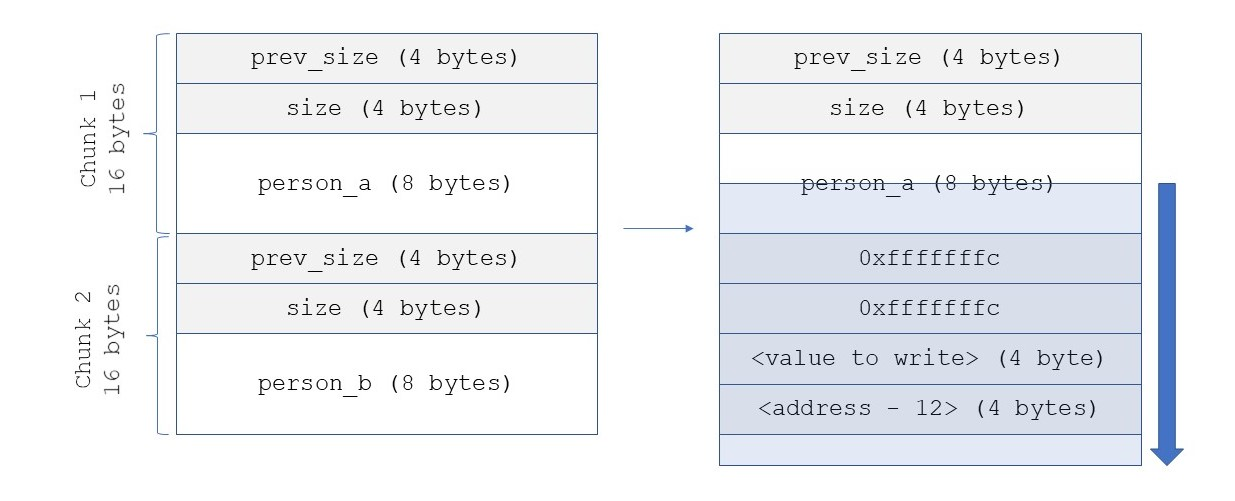
\includegraphics[width=\textwidth]{2b.jpg}\\
Since the heap is initially empty, \texttt{person\_b} will be allocated right next to \texttt{person\_a}. If we provide a name longer than  character for \texttt{person\_a} we can overwrite the metadata of the chunk containing \texttt{person\_b}. The metadata contains two fields, each of which is 4 bytes long. A function pointer is also 4 bytes long. So if the name is $4 + 4 * 2 + 4 = 16$ bytes long, we can use the last 4 bytes to set the function pointer \texttt{person\_b->greet} to be any function we want to execute. \\\\
Heap memory is in general not contiguous (except initially). The heap uses doubly linked lists called free-lists to manage unallocated chunks. Each chunk, whether allocated or not, contains the size of the previous chunk and the size of the currrent chunk in its header, and the last bit of the size field indicates whether the previous chunk is allocated. In addition to these two fields, unallocated chunks also contains in its header \texttt{FD} and \texttt{BK} pointers pointing to adjacent free chunks.\\\\
With older implementations of \texttt{malloc}, we can exploit the allocator by overwriting heap metadata (chunk headers). The high-level idea is to fake a free chunk to trick the deallocator into coalescing two ``free'' chunks using the \texttt{unlink} macro, which simply does \texttt{p->bk->fd = p->fd;} and \texttt{p->fd->bk = p->bk;} to remove the chunk from its original free-list. We can use one of those two write operations to overwrite the address of \texttt{free} to be the address of some malicious code so that the next time any memory needs to be deallocated, malicious code would run instead. \\\\
In the above code example, Suppose \texttt{chunk\_a} contains \texttt{person\_a} and \texttt{chunk\_b} contains \texttt{person\_b}. When \texttt{person\_a->name} overflows into \texttt{chunk\_b}, we can write fake metadata \texttt{chunk\_b->size = -4}. Now, when \texttt{free(person\_a)} is called, the deallocator, following its algorithm, will compute the address of the chunk after \texttt{chunk\_b} to see if a merge is possible, and it will actually get to \texttt{chunk\_b - 4} and it will interpret \texttt{chunk\_b - 4 + 8} which is actually \texttt{chunk\_b -> prev\_size} as the \texttt{size} field of the ``next'' chunk. So if we set \texttt{chunk\_b->prev\_size = 0xfffffffc} then the deallocator will see that the last bit is unset, so it would consider \texttt{chunk\_b} as freed and therefore coalesce \texttt{chunk\_a} and \texttt{chunk\_b} and unlink \texttt{chunk\_b}. We can now utilize the reassignment of linked-list node pointers to write to an arbitrary address. For example, we can put \texttt{<func ptr to free> - 12} in \texttt{chunk\_b->fd} and the address of our injected code in \texttt{chunk\_b->bk}, which will set the pointer to \texttt{free} to point to our code.
\section{}
\section{}
Both ROP and JOP are used to circumvent code injection defense mechanisms because they only utilize existing code in the exploited program. Both kinds of attacks are based on manipulating program execution by chaining together snippets of code ending in some control flow instruction (\texttt{ret} for ROP, \texttt{jmp} for JOP). The main difference between ROP and JOP is that \texttt{ret} gadgets can naturally return back the control based on the content of the stack, but \texttt{jmp} is uni-directional, so it was previously thought to be difficult for attackers to maintain control. However it has be proven that with an additional dispatcher gadget to govern control flow among various jump-oriented gadgets such attacks are feasible.
\end{document}
